Graphical Processing Unit (GPU) devices were originally designed to render graphics efficiently.
%
However, with their multi-threading capabilities providing unprecedented computational speed, they have expanded beyond their original use case.
%
Nowadays, GPUs are essential in general-purpose computing, particularly for applications that handle massive amounts of data and require parallelization to manage their heavy workloads.
%
With GPUs being used for general-purpose computing, everyday users can also benefit from their extensive hardware parallelization.
%
For example, tasks like encryption/decryption of large data sets and training an LLM model can be carried out more efficiently with the use of GPUs.

Many of these applications involve confidential data. 
%
For example, LLMs may work with a large set of personal data based on the application, e.g., medical data.
%
In cryptography, both the plaintext and the encryption key are confidential.
%
It is important to show that this secure information is not leaked to public output channels, either directly or through so-called side channels such as timing, power consumption, or memory usage.
%
Unfortunately, prior work~\cite{AESattack, jiang2019TACO, jiang2019thesis, pustelnik2024arxiv} has revealed several security vulnerabilities in GPU kernels, including leaking via a timing channel rooted in the unique memory access pattern of GPUs across multiple threads to shared and global memory~\cite{AESattack, jiang2019TACO, jiang2019thesis}.
% Unfortunately, prior work has revealed several security vulnerabilities in GPU kernels, ranging from leaking via a timing channel rooted from the unique memory access pattern of GPUs across multiple threads to shared memory (?) and register spills rooted from scheduling of multiple shaders (applications?) on a single GPU.

In addition to security vulnerabilities within a single GPU application, even more vulnerabilities arise when multiple, non-mutually-trusting applications run on a single GPU.
%
This is often the case, as it is not always efficient to allocate an entire GPU to a single application when only a fraction of the processing power will be utilized.
%
Recognizing this, datacenter providers have started to provide GPU-as-a-service (GaaS) on cloud.
%
For instance, Google's Kubernetes Engine allows for the sharing of a GPU among up to 48 tenants, while Microsoft has incorporated GPU paravirtualization into the Hyper-V Hypervisor, enabling VMs to share a single GPU.
%
Recent research~\cite{pietro2016TECS,hayes2017usenix} has revealed security vulnerabilities in GPUs rooted in the scheduling of multiple applications on a single GPU and lack of proper memory isolation between them.

The field of Information Flow Control (IFC) aims to guarantee that secure
data within a program cannot leak to public output channels in unintended
ways.
%
There has been a wide array of prior work on language-based techniques for
guaranteeing IFC on CPU programs.
%
However, a study of \emph{GPU vulnerabilities} from the perspective of language-based security is missing from the literature.
%
Research on CPUs cannot be directly applied here, mainly because the memory model and parallelism paradigm are different from CPUs; the unique memory and execution models of GPUs  introduce new attacker models, including new side-channel attacks.

% Recent research has revealed several security vulnerabilities in GPUs.
%
% \farzaneh{prior work on GPU}
%

% In addition to security vulnerabilities within a single GPU application, even more vulnerabilities arise when multiple, non-mutually-trusting applications run on a single GPU.
% %
% This is often the case, as it is not always efficient to allocate an entire GPU to a single application when only a fraction of the processing power will be utilized.
% %
% Recognizing this, datacenter providers have started to provide GPU-as-a-service(GaaS) on cloud.
% %
% For instance, Google's Kubernetes Engine allows for the sharing of a GPU among up to 48 tenants, while Microsoft has incorporated GPU paravirtualization into the Hyper-V Hypervisor, enabling VMs to share a single GPU.
% also serve as a powerful platform for accelerating
% ubiquitous, non-graphical rendering tasks.
% GPUs' ability to execute thousands of threads concurrently makes them essential in general-purpose computing.

% Here we look at two main category of attacks.
%
% However, its memory layout and the cost properties introduce vulnerabilities, e.g., shared memory bank conflicts.
%

%

We propose a language-based approach for understanding and addressing information flow vulnerabilities in GPU applications, addressing direct and side channels within a single application as well as leaks between multiple applications sharing a GPU.
%
Our approach allows for understanding the fundamentals of security in this new concurrency paradigm and provides provable security guarantees.
%
With this fundamental understanding, it will also be more feasible to incorporate our GPU approach with prior approaches to language-based security for CPUs to provide end-to-end security for applications that, like many of the real-world applications described above, involve both CPUs and GPUs.


\subsection{Intellectual Merit}
The goal of this work is the first language-based security analysis for general-purpose GPU programs.
%
We consider two main forms of attacks, both enabled by the unique memory
layout and execution models of GPUs.
%
While the performance and security pitfalls of the GPU programming model are well-documented empirically, very little prior work has aimed to formalize this model to gain a better understanding of it, let alone from a security perspective.
%
As part of this work, we will gain a better formal understanding of this increasingly crucial computing platform.
%
This formal understanding will come in the form of Information Flow Control type systems for GPU programs, program logics for proving properties about memory and other resource usage of GPU programs, and operational semantics that model the execution of multi-program GPU systems and can be further enriched by a dynamic security monitor.
%\farzaneh{added the dynamic security monitor to the above sentence. Is it ok?}
% \stefan{I specialize to CUDA here. I think this is a good place to do it, let me know if you disagree.}

In the text and examples of this proposal, we focus on CUDA, a general-purpose GPU programming framework developed by NVIDIA.
%
CUDA is extremely widely used and is also the basis of most of the prior work on formally understanding GPU execution, so it is a good starting point for our work.
%
However, because the memory and execution models are largely a result of the design of GPU hardware, the ideas explored in this work will be applicable to other GPU programming frameworks.

We now briefly outline the main thrusts of the proposed research.
%
The descriptions here are necessarily at a fairly high level because we defer until Section~\ref{sec:background} the discussion of the specific characteristics of GPUs that lead to the security vulnerabilities.

\paragraph{Thrust 1. Passive attacks}
In Thrust 1, we consider passive attacks that exploit the correlation between memory access patterns and access time: in CUDA, the GPU attempts to combine memory accesses from multiple threads into fewer hardware operations, but the amount of time this saves depends on the memory access patterns (e.g., the indices of an array accessed by each thread).
%
In this attack, the attacker does not interfere with the victim process but is a passive observer who observes the computation time. 
%
From the computation time, the attacker can deduce the index used for accessing an array stored in memory, since the indices used can trigger performance gains or losses.
%
(See Figure~\ref{fig:th1-attack}(a)-(b).)
% \farzaneh{Talk about related work on correlating timing attacks}
\begin{figure}[h]
    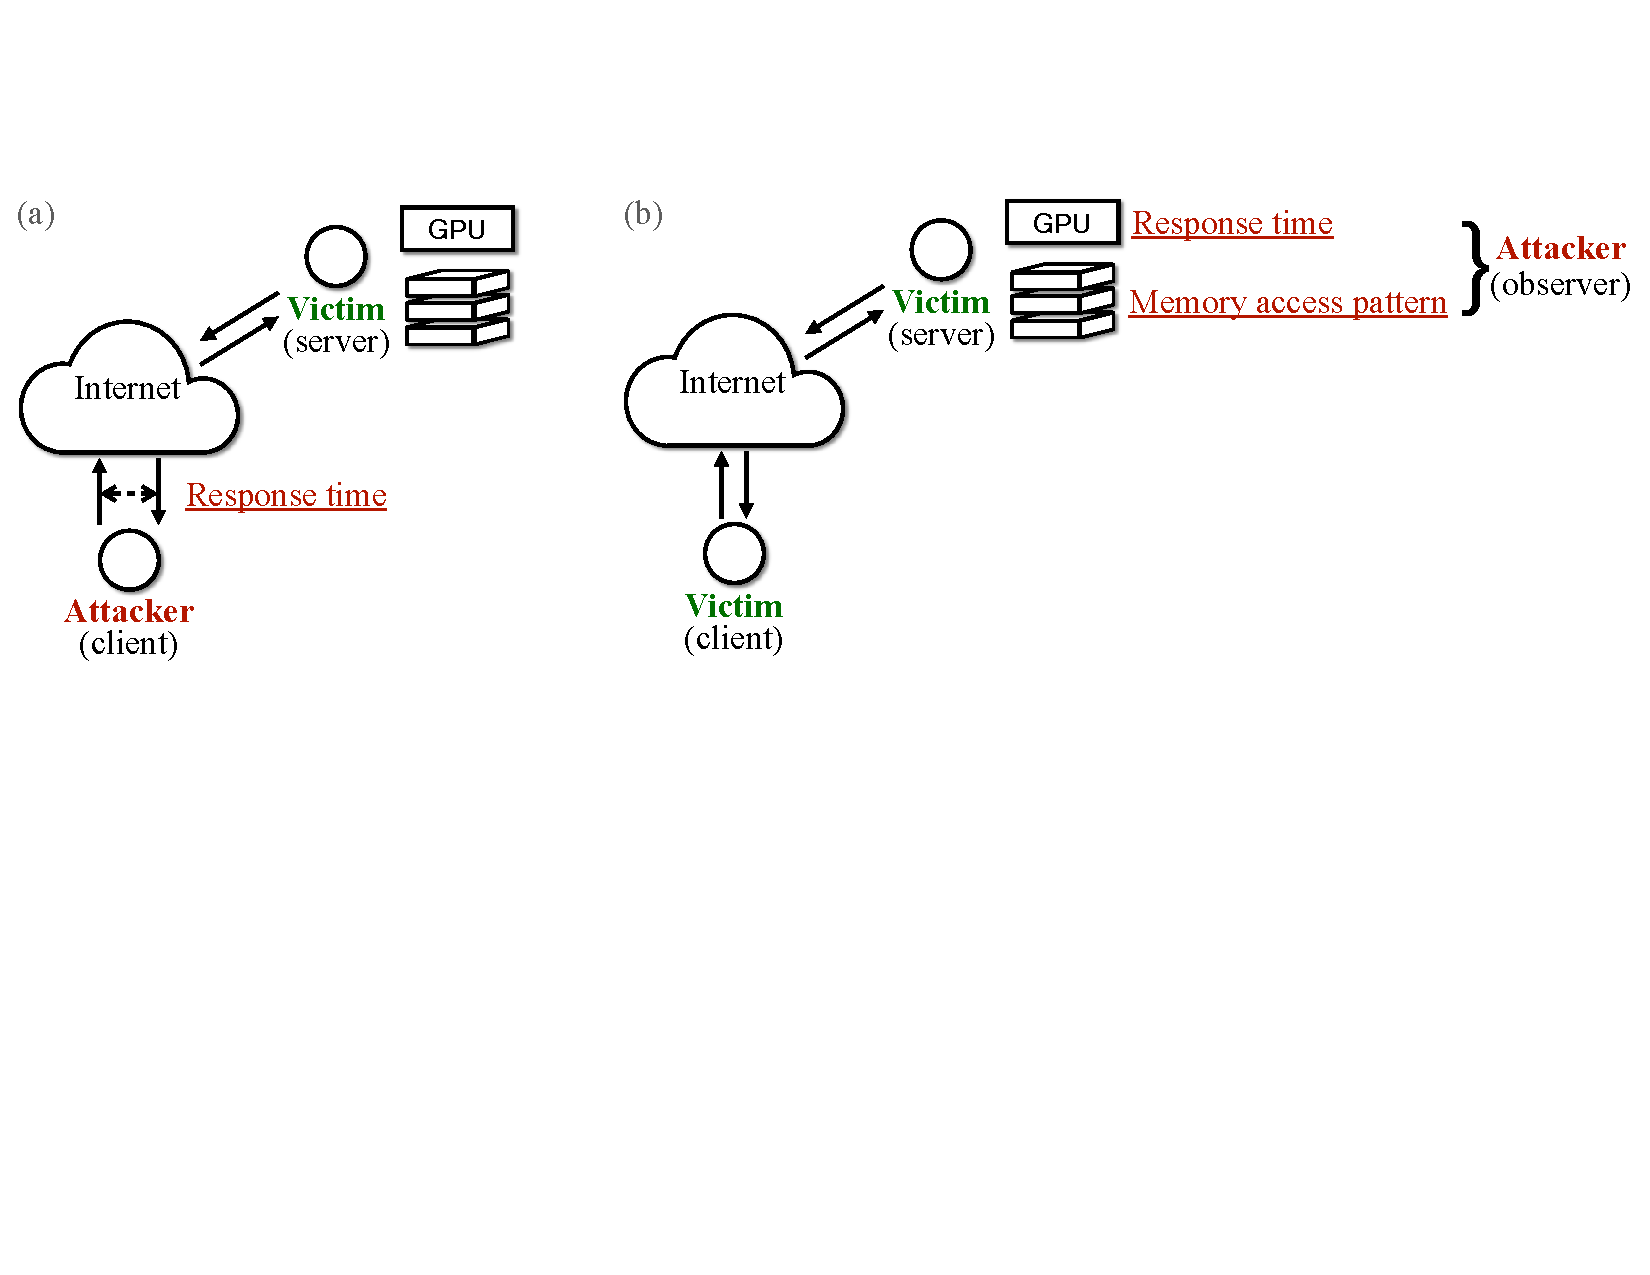
\includegraphics[clip,trim=0 10cm 0 2cm,width=0.72\pdfpagewidth]{figs/thrust1-fig.pdf}
    \caption{Attacker models considered in Thrust 1 \farzaneh{add quantitative?}}
    \label{fig:th1-attack}
\end{figure}

In order to mitigate these timing channel attacks through memory accesses, we propose a relational, resource-aware program logic capable of proving facts about the difference in execution time between two runs of a program.
%
This logic is sufficient to guarantee that execution time is independent of secret input (a security property known as {\em noninterference}), but is quite heavyweight and likely to require some programmer annotation.
%
We additionally develop an IFC type system which tracks the security level of data as it moves through a program and disallows memory accesses that could leak secure information; the type system is necessarily more conservative than the program logic, but much easier to work with in practice and uses the program logic to gain precision at strategic points.

\paragraph{Thrust 2. Active attacks}
In the attacks we consider in Thrust 2, the attacker has their own process in the cloud (as a client), which coexists with the victim process.
%
The victim and attacker both use the GPU server on the cloud.
%
The attacker, through leaks caused by lack of proper isolation for shared and  global memory locations between processes, can gain access to the contents of the victim process's address space that may have been inadvertently left behind.
% through leaks caused by the reuse of the registers and memory locations between processes, can gain access to the contents of the victim process's address space.
%
(See Figure~\ref{fig:th2-attack}.)
\farzaneh{we only talk about shared and global memory in Thrust 2. I dropped registers from above.
}
\begin{figure}[h]
    \centering
    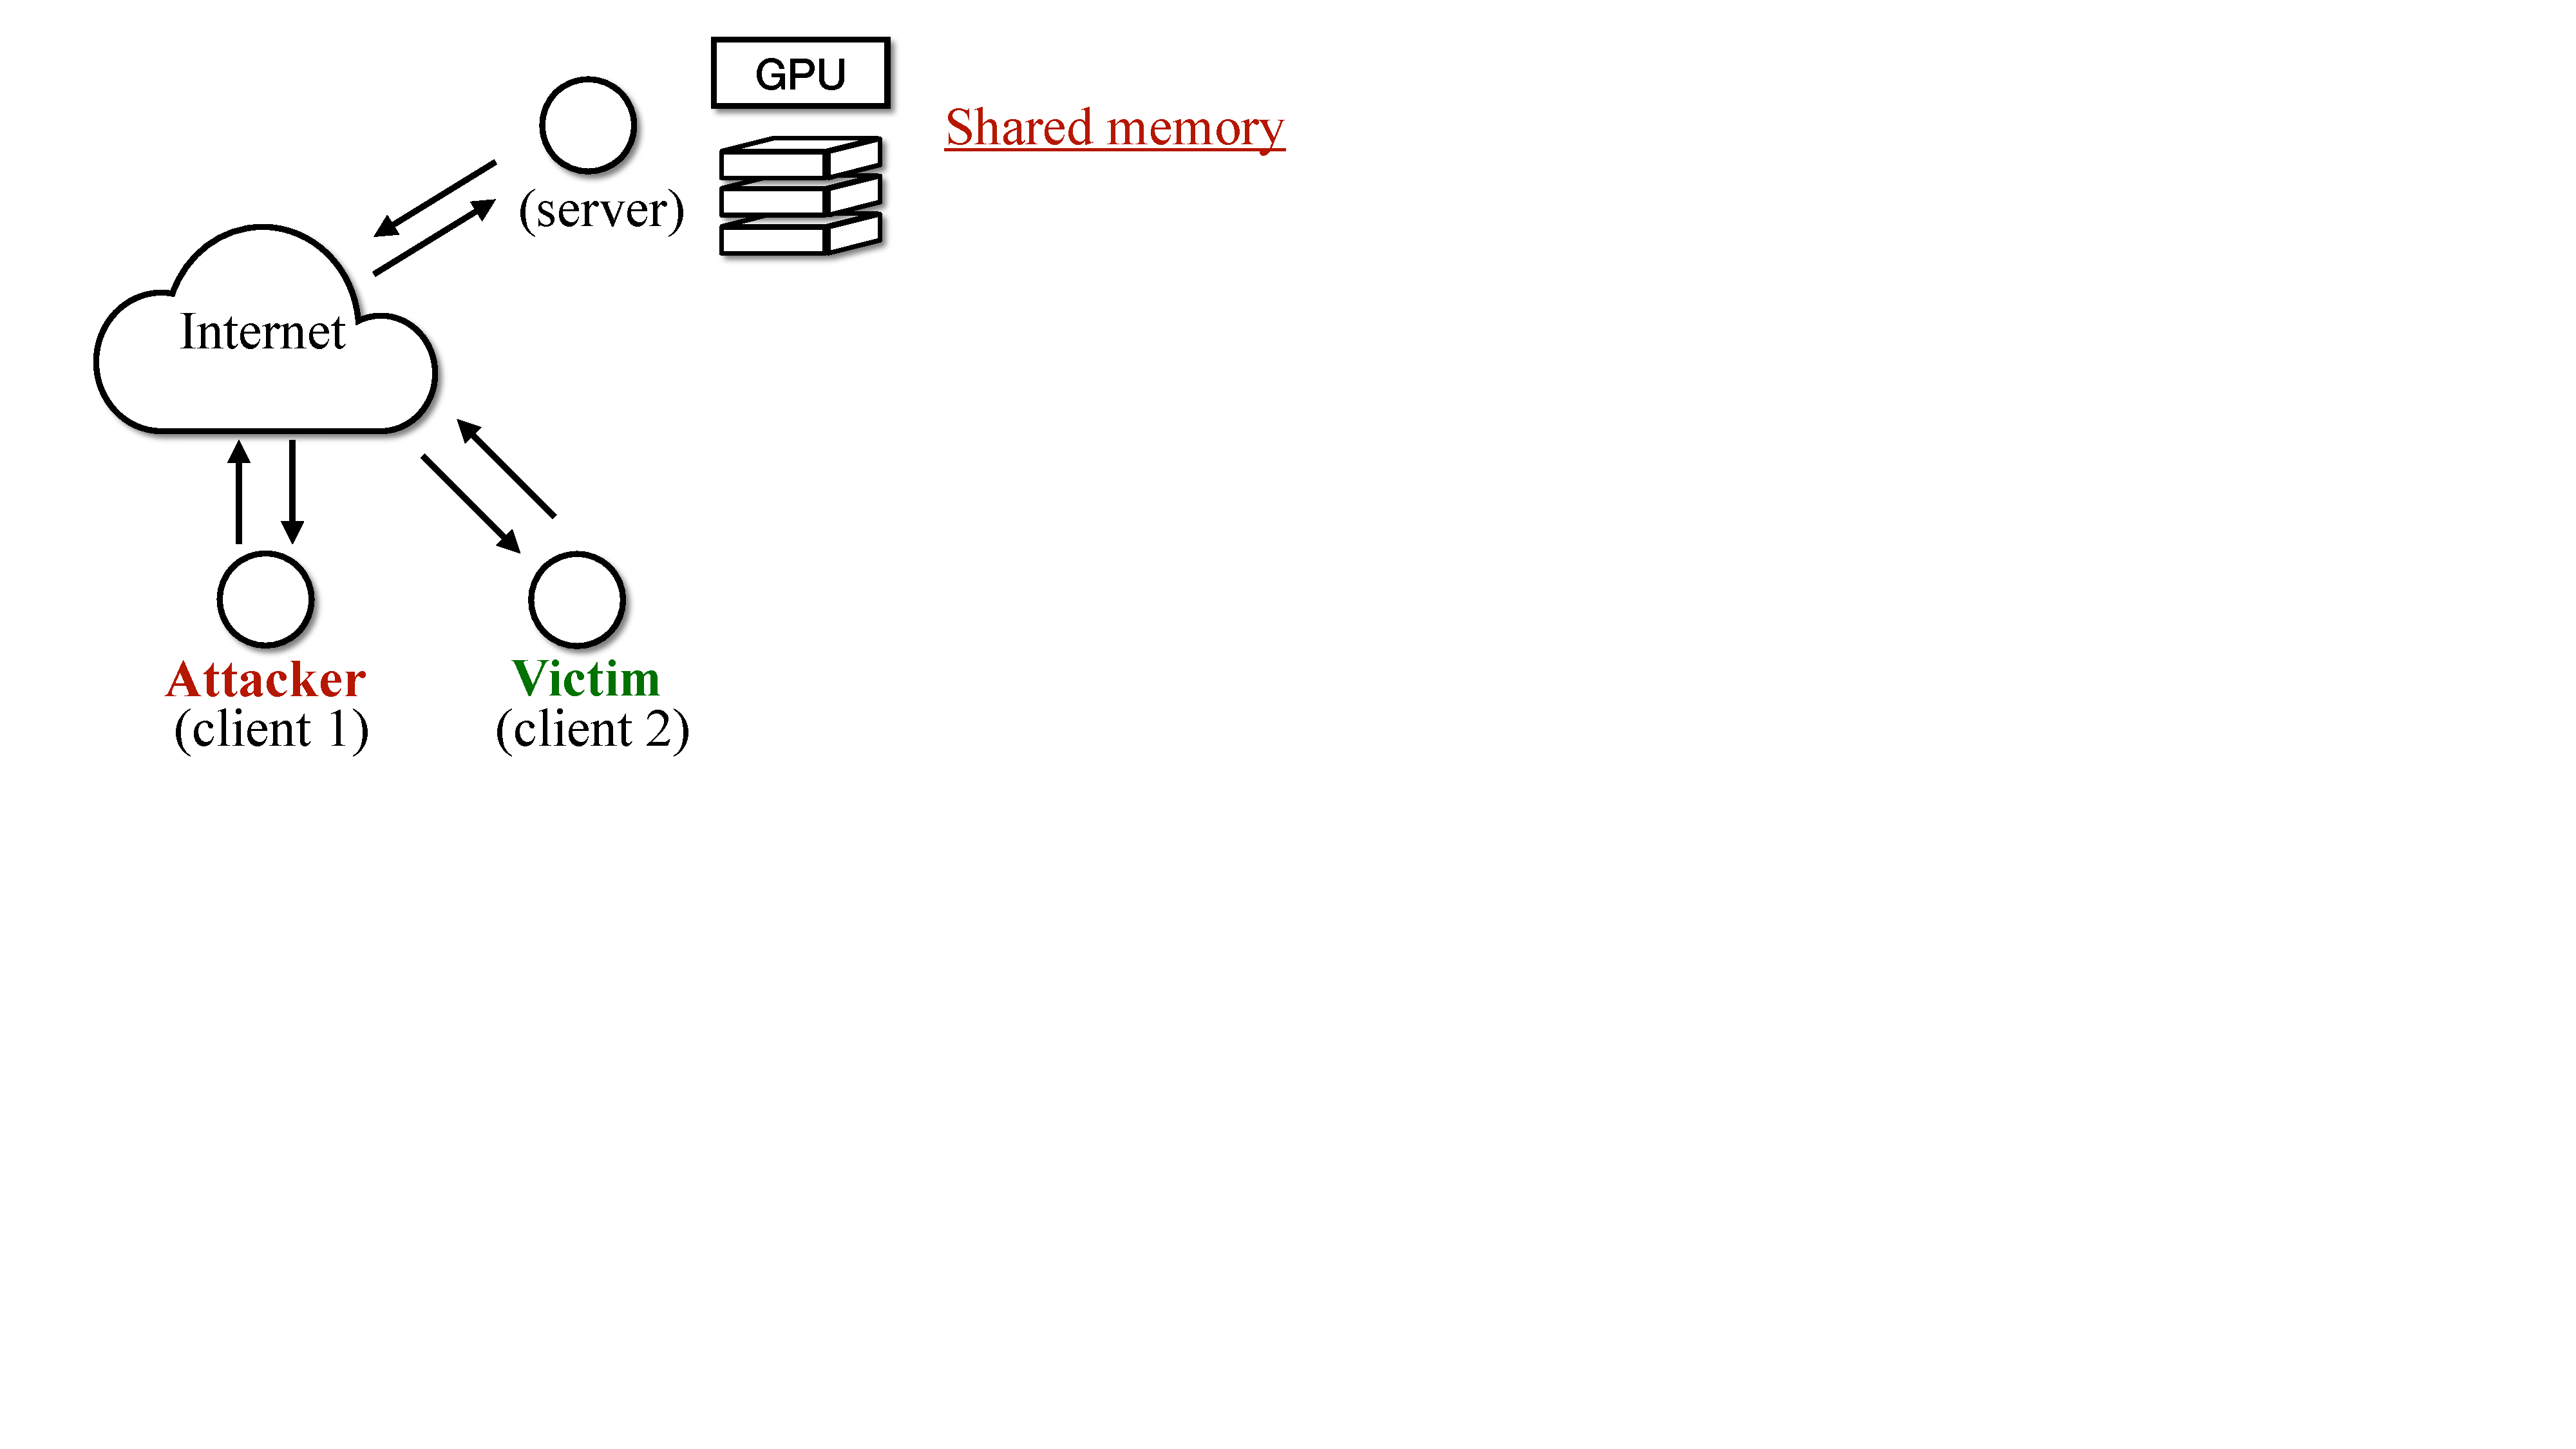
\includegraphics[clip,trim=0 17cm 10cm 0cm,width=0.72\pdfpagewidth]{figs/thrust2-fig.pdf}
    \caption{Attacker model considered in Thrust 2 \farzaneh{add more}}
    \label{fig:th2-attack}
\end{figure}

To prevent such attacks, we ensure that the victim process does not leave behind secure information in the shared and global memory. We acheive this by designing a flow-sensitive taint tracking system that captures the flow of sensitive data throughout the program and memory locations statically via taint levels.
%
While this static approach is low-cost, it only provides an over-approximation of the security guarantees. 
We address the limitations of the static analysis approach by incorporating a hybrid method that combines both static and dynamic taint tracking.

% \stefan{Talk about what we do.}


\paragraph{Thrust 3. Case study}
In Thrust 3, we implement two case studies (AES encryption and a Large Language Model application), which have been previously shown to be vulnerable to the attacks described in the first two thrusts.
%
We will show that these vulnerabilities are detected by the type system and program logic of Thrust 1, both in theory and using the implementations of the type system and program logic that we will build as part of the thrust.
%
We will then demonstrate the Thrust 2 vulnerabilities by implementing an attacker process that can run alongside the case study applications and take advantage of information leaks.
%
Finally, we plan to create patched versions of the two case studies and demonstrate that the security vulnerabilities have been mitigated.


\subsection{PI Qualifications}

PIs Derakhshan and Muller will work closely together to complete the objectives
of the proposal.
%
Both PIs are in the Programming Languages group at Illinois Tech, and have been
working closely together since PI Derakhshan joined the faculty, including
coadvising a number of students, one of whom has begun preliminary studies
on the proposed work.
%
{\bf PI Derakhshan} is an expert on language-based security.
%
She and her collaborators have designed flow-sensitive IFC-type systems for concurrent message-passing processes and proved progress-sensitive noninterference for well-typed processes, also ruling out timing attacks that exploit the relative order of messages~\cite{derakhshan2021LICS, van2024ecoop,derakhshan2024ecoop}.
%
She and her collaborators have also developed a formal framework for end-to-end verification of security properties for Trusted Execution Environments in the context of multiple CPU cores~\cite{derakhshan2023CSF}.  
%
{\bf PI Muller} is an expert in static resource analysis, and has previously
conducted a successful NSF-funded study on static resource analysis for CUDA.
%
As part of this work, PI Muller and his students and collaborators
developed an operational semantics for CUDA as well as a resource-aware
program logic (and an OCaml implementation of it) for predicting the impact
on execution time of CUDA performance characteristics such as the ones
that lead to the described vulnerabilities~\cite{MullerHo21}.
%
We plan to use this logic and its implementation as a starting point for
our work.
\farzaneh{Some of the citations are missing from your paragraph?}
\stefan{Those are all actually from the same paper. Does it look bad to just
cite one?}
\subsection{Broader Impacts}

With the rise of machine learning and large language models and the recognition that the parallel performance of GPUs is necessary to achieve the required scaling, GPU computing has become a multi-trillion-dollar industry.
%
However, a number of recent high-profile leaks have made consumers understandably wary of the use of their private data.
%
Understanding the security risks of GPU computing and how to mitigate them is of paramount importance to the continued success of this burgeoning area.
%
In addition to the clear benefits to society, this project will provide numerous opportunities for student research, including undergraduate research, at Illinois Tech, an R2 research university with a demographically and economically diverse student body.
%
We discuss the broader impacts of the proposal in more detail in Section~\ref{sec:impacts}.
